\section{Modelo de interacción de documentos}

\par En la figura \ref{fig:did} mostramos cómo fuimos relacionando las entidades para formar documentos con suficiente información como para satisfacer las consultas necesarias y no perder información en el medio.
La idea general es poder tener los siguientes documentos:
\begin{itemize}
  \item \textbf{Cliente}: posee información del cliente, junto con su historial de atracciones visitadas.
  \item \textbf{Evento}: posee información de una evento y las visitas que tuvo (entradas registradas en la base de datos original).
  \item \textbf{Parque}: posee información del parque, las visitas que tuvo (entradas registradas en la base de datos original) y un listado de sus atracciones, junto con el historial de visitas.
  \item \textbf{Factura}: posee los datos de la factura y un listado de referencias a las entradas que se incluyen en ella.
\end{itemize}

\begin{figure*}[ht]
  \hspace*{-1.5cm}
  \begin{subfigure}{1.2\textwidth}
    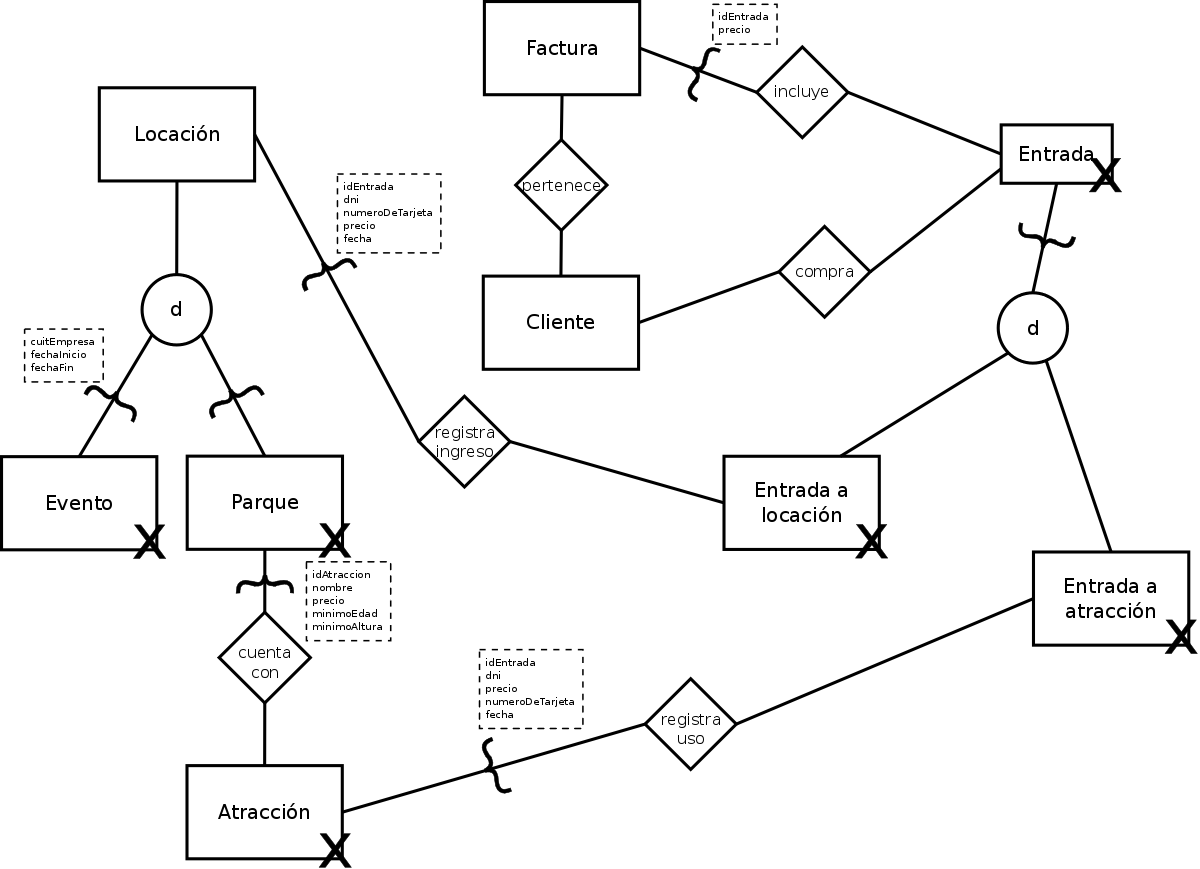
\includegraphics[width=\textwidth]{src/did.png}
  \end{subfigure}
  \caption{Diagrama de interacción de documentos.}
  \label{fig:did}
\end{figure*}
